\chapter{Un transmisor ISDBT implementado en GNU Radio}

\section{Generalidades del Transmisor}
Por ejemplo algunas
\section{El flujo de datos en GNU Radio}

Para el desarrollo de los bloques de gr-isdbt-tx, fue necesario comprender el modo en el que los datos se mueven entre bloques en GNU Radio. El motor del programa realiza llamados de forma periódica a los bloques en el flowgraph, dependiendo de la cantidad de muestras que tenga en cola para procesar en cada bloque, y de la tasa de muestras que busque mantener constante a traves del sistema, le comunica a cada bloque, la cantidad de datos que necesita que le dejen en salida.  

Al momento de crear un nuevo bloque, debemos especificar en la firma de la función, los parámetros necesarios para que el motor central pueda controlar de flujo de datos de nuestro nuevo bloque. Para realizar esto, se utilizan ciertos parámetros, precargados en la estructura de clases de los bloques, orientados a la entrada/salida de datos, estos son,  noutputitems y ninputitems. 

Mediante estas variables, el motor de procesamiento puede obligar a los bloques a ejecutarse mas de una vez en cada llamado, pues exige la cantidad de salidas que necesita para mantener la tasa. Para esto, le notifica al bloque en la variable noutputitems, la cantidad de “tandas” de datos que la instancia actual del bloque necesita devolverle al motor de procesamiento para mantener la tasa. 

La variable ninputitems, mantiene el control de la cantidad de datos que hay en cada uno de los puertos de entrada. Y utilizándola como variable, podemos especificar cuantos datos de entrada precisamos consumir para obtener un dato en el puerto de salida.

Esta operación depende bastante de la naturaleza del bloque, por ejemplo, en los bloques síncronos, se sabe de antemano que la tasa de muestras se mantendrá constante, por lo que alcanza con especificar el tipo y la cantidad de muestras que atravesaran el bloque en una ejecución. 

Los bloques de tipo general, son mas complicados, pues es necesario especificar explícitamente la relación entre la cantidad de muestras a la entrada y a la salida. Este control de flujo se realiza desde un método, precargado en la clase con la que se crea el bloque, denominado forecast.

\section{Obtencion de los TSP por capa}

Como se explico anteriormente, en un solo flujo de transporte coexisten paquetes pertenecientes a las distintas capas de transmisión, sino que también están las tablas de información, y los paquetes nulos para mantener el flujo de datos constante. 

Es necesario separar al principio del transmisor, esta información, para procesarla individualmente cada capa, afín de lograr mantener los programas contenidos en la misma en un mismo flujo, pues como vimos, las capas pueden tener distintas modulaciones y distintos retardos. 

Cada paquete tiene en su encabezado IIP, un parametro denominado \textit{layer\_information}, que contiene información sobre la capa de transporte a la que pertenece. El parametro ocupa los primeros cuatro bits del segundo byte del encabezado del TSP, y se decodifica según la siguiente tabla

\begin{table}[h!]
	\centering
	\begin{tabular}{|c|c|}
		\hline
		\textbf{Valor $b_{7}b_{6}b_{5}b_{4}$} & \textbf{Capa}\\
		\hline
		0000 		& Null TSP\\
		\hline
		0001 		& Capa A\\
		\hline
		0010 		& Capa B\\
		\hline
		0011 		& Capa C\\
		\hline
	\end{tabular}
	\caption{\label{Identificador de capa para TSP} Par\'ametro indicador de capa en el IIP.}
\end{table}

El primero de los bloques de gr-isdbt-tx, es un bloque que se encarga de realizar esta tarea. Dado que conocemos de antemano la cantidad de TSPs que estan contendios en un cuadro multiplex de nuestro BTS de prueba, definimos un bloque con un puerto de entrada y tres puertos de salida. En cada ejecucion, se recorre un cuadro multiplex, analizando para cada uno de los TSP el parámetro \textit{layer\_information}, decodificamos a que capa pertenece, y se enrutan según corresponda. 

Entendemos que la implementación que presentamos de este bloque, existen cosas a mejorar. No las incluimos en este release del código por cuestiones de tiempo. De primera mano, la cantidad de TSP por cuadro multiplex podría ser calculada en tiempo de ejecución, para el BTS que el usuario quiera usar en ese momento, al igual que la cantidad de paquetes de cada capa. Hoy esos parámetros están fijados, y eso limita la robustez del transmisor. Discutiremos estos temas mas a fondo en el capitulo 7.

\section{Codificaciones de Canal}

	\subsection{Reed Solomon}
La norma ISDBT utiliza una implementación exactamente similar a la de DVB-T del codificador Reed Solomon. En cada TSP se sustituyen los últimos 16 bytes del IIP por la palabra de redundancia de un codigo RS(204,188). Para lograr esta distancia, lo que se hace es llevar el payload hacia un tamaño mas grande, agregando 51 bytes en 0 al comienzo del TSP. Luego, el nuevo payload de 239 bytes, se inyecta en un codificador RS(255,239). 

El cambio de tamaño se realiza principalmente para utilizar un algoritmo mas eficiente. Una vez obtenida la palabra codigo del mismo, se remueven los primeros 51 bytes nulos, y obtenemos el codigo RS(204,188) que entra en el tamaño de un TSP, y ademas es capaz de corregir errores hasta de 8 bytes. 

Para la implementacion de esta funcionalidad en ISDB-T, no fue necesario desarrollar ningun bloque. Dentro de los complementos de GNU Radio esta el paquete gr-dvb \cite{gr-dvb} (originalmente un proyecto de terceros, que en 2015 fue incorporado al repositorio oficial de GNU Radio), que contiene los bloques necesarios para implementar tanto un transmisor como un receptor bajo la norma DVB. Al compartir el codificador Reed Solomon con ISDBT, basto con utilizar el bloque de gr-dvb.

\begin{figure}[h!]
	\centering
	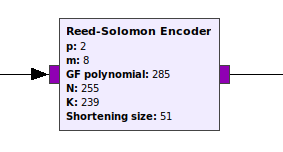
\includegraphics[scale=0.5]{figuras/cap05/RSencoder}
	\caption{\label{f:RSencoder} Bloque Reed Solomon Encoder de gr-dvb.}
\end{figure}

En la figura 5.1, mostramos el bloque y la configuracion parametrica del mismo, tal cual se implemento en gr-isdbt-tx. Los parametros \textbf{p}, \textbf{m} y \textbf{GF polynomial} son los que configuran el polinomio generador que es la base del algoritmo. Para lograr el polinomio generador del algoritmo para RS(255,239), debemos utilizar el polinomio:

\begin{gather*}
	p(x) = x^8 + x^4 + x^3 + x^2 + 1
\end{gather*}

	\subsection{Viterbi}
	Otro de los códigos de canal implementados por ISDBT es el código Viterbi. Este código, es  convolucional con puncturing, su codigo madre tiene una tasa de $\frac{1}{2}$ y constante $k = 7$, lo que permite obtener en salida datos codificados a cualquier tasa m/n en transmisión, sin aumentar la complejidad de la decodificación en recepción. 
	
	Esto sucede, porque tanto el lado transmisor como el receptor, conocen la llamada matriz de puncturing. En esa matriz, se especifica para cada tasa de código buscadas, los bits redundantes que serán eliminados al transmitir, para lograr la tasa deseada. Vale recordar que estos bits deben ser reingresados por el decodificador en recepción, pues de lo contrario aumentaría fuertemente la complejidad de la decodificación.
	
	\begin{figure}[h!]
		\centering
		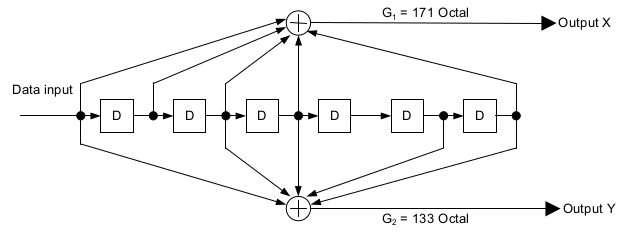
\includegraphics[scale=0.5]{figuras/cap05/viterbi}
		\caption{\label{f:viterbi} Circuito del codigo madre del Viterbi que implementa ISDBT.}
	\end{figure}
	
	Agregar este tipo de códigos a la cadena de transmisión, aumenta la resistencia ante las perdidas y mantiene una tasa de bits constante, lo que colabora con el mantenimiento del sincronismo del sistema.
	
	DVB utiliza el mismo código en su cadena de transmisión, con los mismos parámetros, por lo que en gr-isdbt-tx, no fue necesario realizar un desarrollo del bloque sino que reutilizamos el existente en gr-dvb. 
	
	\begin{figure}[h!]
		\centering
		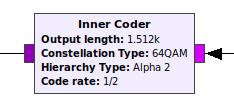
\includegraphics[scale=0.5]{figuras/cap05/inner}
		\caption{\label{f:inner} Bloque de gr-dvb que implementa el codificador Viterbi.}
	\end{figure}
	
\section{La modulacion}

Para resolver la modulación en nuestro transmisor, decidimos crear un solo bloque que resuelva en conjunto los problemas de interleaving de bits y modulacion. Esto resulto bastante conveniente, pues basto con crear una variable que contenga un selector de modulacion, y en base a el se crean una serie de colas, cuyos tamaños responden a lo explicado sobre interleaving en el inciso 5.7.

\begin{figure}[h!]
	\centering
	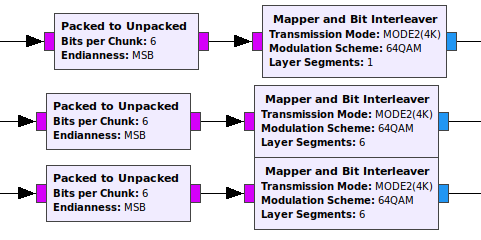
\includegraphics[scale=0.5]{figuras/cap05/modulacion}
	\caption{\label{f:modulacion} Implementacion de la modulacion e interleaving a nivel de bits en gr-isdbt-tx.}
\end{figure}


El problema que nos encontramos en esta etapa, fue el de particionar la informacion en un byte, pero conservar el resto. Un ejemplo claro de esto se da cuando la modulacion es \textit{64-QAM}, pues cada simbolo en este caso se construye con 6 bits. Ahora, el parseo de datos entre bloques, GNU Radio lo hace encapsulados en datos de tipo \textit{byte}. Por lo tanto, necesitabamos una forma de resolver el problema de separar 6 bits utiles de un dato, y guardar los 2 siguientes para el proximo simbolo. En principio, no pareceria ser un problema tan grave, pero podria pasar que los 2 bits que nos quedan pendientes, se correspondan con un simbolo que se construira en una proxima llamada al metodo modulador del objeto "bloque mapper". A nivel de programacion, esto implica que la memoria volatil de la instancia del objeto, se borra, por lo que habria que utilizar algun almacenamiento que permanezca en memoria estatica, y actualizarla en cada simbolo que se procesa.

Recorrer ese camino nos pareció ademas de muy laborioso, poco eficiente en terminos de CPU. Encontramos la solucion en un conjunto de bloques propietarios de GNU Radio, que lo resuelven de manera eficiente. Los bloques \textit{Packed to Unpacked} nos resuelven el problema. Basta con tener en cuenta a la hora de utilizar el tranmisor, definirle el parametro de \textit{Bits per Chunk} de forma consistente con la modulacion que se este utilizando. 

\begin{table}[h!]
	\centering
	\begin{tabular}{|c|c|}
		\hline
		\textbf{Modulación} & \textbf{Bits por símbolo}\\
		\hline
		QPSK		& 2\\
		\hline
		16-QAM 		& 4\\
		\hline
		64-QAM		& 6\\
		\hline
	\end{tabular}
	\caption{\label{Bits por simbolo segun modulacion} Bits por símbolo según modulación.}
\end{table}

A la salida de los bloques \textit{Bits per Chunk}, tendremos un byte completo de 8 bits, pero rellenado con la cantidad de bits requerida por la modulación, comenzando por el bit mas significativo.  Esto nos permite normalizar la recepción de datos del bloque modulador, para cada caso, sabremos perfectamente como esta compuesto el byte de datos. 

Una vez allí, alcanza con crear una cola con el retardo correspondiente, y enrutar los bits hacia la misma de forma ordenada. La secciona de modulación del bloque, funciona de la siguiente manera. 

Se obtiene de la cola los bits a procesar, y se arma, manteniendo el orden especificado en la norma, una palabra de N bits, donde $N={2,4,6}$ según corresponda en la tabla \tablename{Bits por simbolo segun modulacion}. Una vez formada la palabra, se re interpreta como un numero decimal, y se busca en un arreglo el complejo que se corresponda con la palabra recién formada. Esta información se obtiene de la tabla   

\section{El uso de los entrelazamientos}

\subsection{Entrelazamiento frecuencial}

El entrelazamiento frecuencial consiste en permutar las portadoras de un s\'imbolo OFDM en el dominio de la frecuencia. Dada la caracter\'istica de ISDB-T de utilizar un gran n\'umero de portadoras, ocurre que frente a canales selectivos en frecuencia se pueden ver afectadas una cantidad importante de portadoras consecutivas, con lo cual la capacidad de correcci\'on de los c\'odigos resultar\'ia superada.

Realizando un entrelazamiento frecuencial las portadoras que pudieran verse afectadas en un canal selectivo son desentrelazadas en recepci\'on y, por lo tanto, los errores que pudieran haber quedan distribu\'idos facilitando la tarea de los c\'odigos correctores.

El procedimiento del entrelazamiento en ISDB-T se divide en dos etapas: el \textit{enterlazamiento inter-segmentos}, y el \textit{entrelazamiento intra-segmentos }.

Primero se separan los segmentos en tres grupos: los destinados a recepci\'on parcial (\textit{one-seg}), los que utilizan \textit{modulaci\'on coherente}, y por otro lado los que utilizan \textit{modulaci\'ion diferencial}. Como en el caso de \textit{gr-isdbt-tx} s\'olo se utiliza modulaci\'on coherente, los caminos que pueden tomar los segmentos son \'unicamente dos.

Posteriormente viene la etapa de entrelazamiento inter-segmentos. Precisamente consiste en intercalar las portadoras entre los segmentos que comparten la modulac\'on. Para el segmento destinado a la recepci\'on parcial este proceso no tiene sentido, por lo cual pasa directamente a la etapa de enterlazamiento intra-segmento.

El entrelazamiento intra-segmento se realiza permutando las portadoras de cada segmento entre s\'i. Se comienza por rotar las portadoras de acuerdo a la siguiente expresi\'on:

Luego se realiza una aleatorizac\'on que est\'a determinada por \textit{Look Up Tables} que dependen del modo de transmisi\'on y puden consultarse en la referencia \cite{bb}.

\subsection{Entrelazamiento temporal}

\section{Entrelazamiento de bits}

Este bloque tiene a cargo esencialmente dos grandes tareas, primero entrelazar los bits que le ingresan provenientes de una determinada capa jerárquica dando lugar a un nuevo flujo de bits entrelazados. Luego estos bits son agrupados para formar símbolos complejos según la modulación que tenga la capa.

El proceso de entrelazamiento se lleva a cabo aplicando retardos definidos según la modulación. Esto supone utilizar una estructura de colas paralelas FIFO de distinto tamaño en las cuales se va colocando de a un bit a la vez. Una vez que se coloca un bit en cada cola, en el otro extremo se forma un complejo extrayendo el último bit de cada cola.

Inicialmente cuando se enciende el sistema se tendrá un transitorio con datos inválidos como producto del contenido de las colas previo al momento de que se inicializa el sistema. Esto no es inconveniente puesto que el receptor descarta esos datos y se sincroniza en un comienzo de frame válido.

Entrelazar utilizando esta mecanismo de colas de retardos variables implica agregar un retardo total correspondiente al camino más largo que deben atravesar los bits, es decir un retardo de 120 símbolos complejos. Según la modulación que utilice la capa estos 120 símbolos se traducen en un mayor o menor retardo en el tiempo; para QPSK corresponde a esperar que ingresen $120 \times 2$ bits en la entrada, mientras que para 64QAM deben pasar $120 \times 6$ bits.

Con el objetivo de tener un mismo retardo para lograr sincronismo en todas las capas se realiza un \textit{ajuste de atraso}. En ISDB-T los retardos deben ser m\'ultiplos de un s\'imbolo OFDM; para el entrelazamiento de bits el retardo propio del proceso de entrelazamiento sumado al ajuste de atraso debe totalizar dos s\'imbolos OFDM.

El tamano de un s\'imbolo OFDM corresponde a: 
\begin{equation}
N_{OFDM} = m_L \times N_L \times 96 \times 2^{modo-1} \quad \text{bits}
\end{equation}

$N_{OFDM}$ depende de la modulaci\'on de la capa $m_L$, que puede ser 2, 4 y 6 para QPSK, 16QAM y 64QAM respectivamente; la cantidad de segmentos utilizados $N_L$ y por supuesto del modo de transmisi\'on. La soluci\'on implementada en \textit{gr-isdbt-tx} consiste en incrementar los tamanos de las colas de manera que el retardo total sea de dos s\'imbolos OFDM para cada capa. Por lo tanto para tener el retardo deseado los tamanos de las colas deben ser:

\begin{equation}
Q_i = q_i + \dfrac{2 \times N_{OFDM} - 120 \times m_L}{m_L} = q_i + N_L \times 96 \times 2^{modo-1} - 120
\end{equation}

\begin{figure}[!h]
\centering
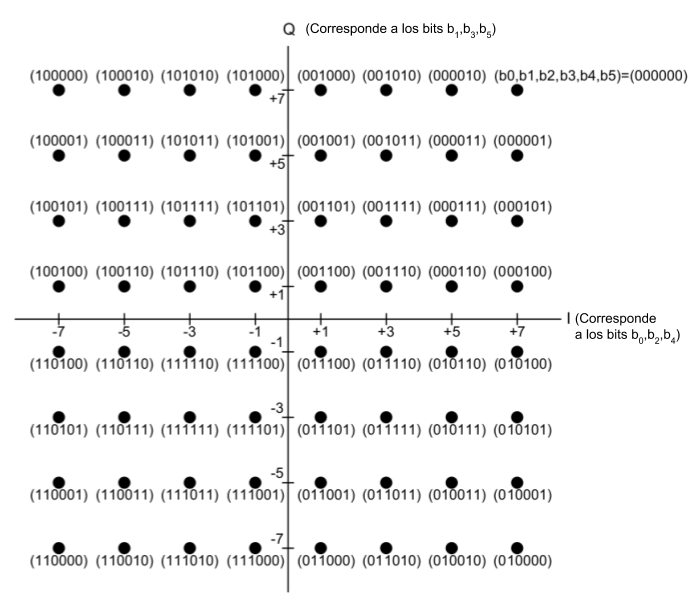
\includegraphics[scale=0.5]{figuras/cap05/constelacion_64QAM}
\caption{\label{f:mapeo_64QAM} Mapeo de la constelaci\'on 64QAM.}
\end{figure}

Una vez que son empujados los bits en cada cola, desde el otro extremo se extrae un bit por cola y se mapean en un s\'imbolo complejo de acuerdo a como lo establece la norma. Por ejemplo en la Figura \ref{f:mapeo_64QAM} se muestra c\'omo se realiza este mapeo para la modulaci\'on 64QAM. Por \'ultimo los complejos deben ser normalizados seg\'un un factor de normalizaci\'on que se presenta en la Tabla \ref{t:factor_normalizacion}.

\begin{table}[h!]
\centering
\begin{tabular}{|c|c|}
\hline
\textbf{Modulaci\'on} 				& \textbf{Factor de normalizaci\'on}\\
\hline
QPSK 		& $1/ \sqrt{2}$\\
\hline
16QAM		& $1/ \sqrt{10}$ \\
\hline
64QAM 		& $1/ \sqrt{42}$ \\
\hline
\end{tabular}
\caption{\label{t:factor_normalizacion} Factores de normalizaci\'on para los distintos esquemas de modulaci\'on.}
\end{table}


\section{Formacion de cuadros OFDM}
El cuadro OFDM es una estructura de datos que agrupa los datos de carga \'util, portadoras piloto y señales de control. Tiene todo lo necesario para que un receptor compatible con ISDB-T sea capaz de decodificarlo en flujos MPEG y reproducir la informaci\'on.

Se trata de un conjunto de 204 s\'imbolos OFDM, cada uno de ellos conformado por $13 \times 108 \times 2^{modo -1}$ s\'imbolos complejos. Una de las particularidades del cuadro, es que su estructura tiene posiciones fijas, donde siempre viaja información con las características de la transmisión, y posiciones móviles, en las que viajan portadoras que estiman el efecto que tiene el canal sobre los datos, para poder, con esa información, robustecer al sistema. 

Para cada segmento, la estructura del cuadro tiene su forma particular. En la siguiente figura presentamos un ejemplo para una modulación coherente, basada en un modo de transmisión 1.

\begin{figure}[!h]
	\centering
	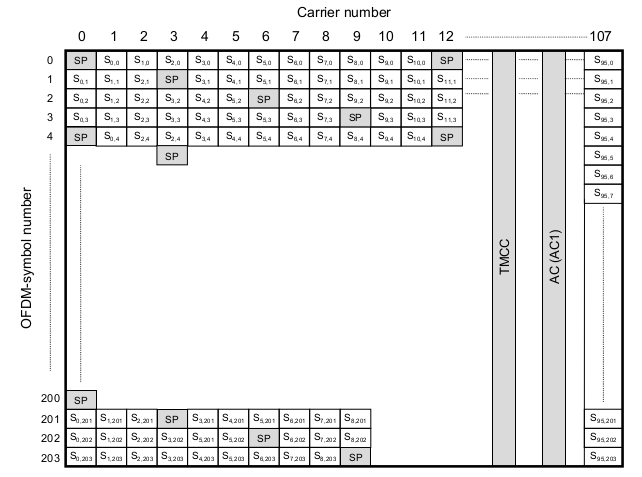
\includegraphics[scale=0.5]{figuras/cap05/ofdm_frame}
	\caption{\label{f:ofdm_frame} Estructura de cuadro OFDM para un segmento, con modo de transmisión 1.}
\end{figure}

A nivel de codigo, la solucion que se implemento en este proyecto para el bloque, es bastante larga. Separamos el bloque en dos momentos, el transitorio y el regimen. Durante el transitorio, esto es, cuando se llama al bloque por primera vez y se crea en la memoria una instancia del mismo, se inicializan todas las variables. Entre ellas estan, la palabra TMCC para todo el cuadro, los valores iniciales de la secuencia PRBS que rige el movimiento de las portadoras SP y algunas variables generales que mantienen conteos de frames para seguimiento. 

En el caso general de un llamado a operar del bloque, la escritura se diseño organizada por simbolos OFDM. En cada llamado al bloque, se completara un simbolo generico. Algunas estructuras de control mantendran el control de los cambios de palabras de control y otras variables. Los parametros genericos de transmision que dependen de parametros como el modo y las constelaciones de cada capa, se resuelven en el transitorio.

\begin{figure}[!h]
	\centering
	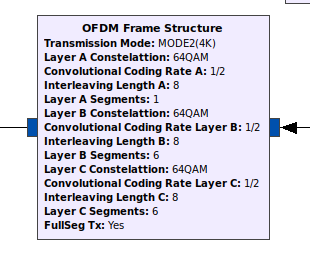
\includegraphics[scale=0.5]{figuras/cap05/bloque_ofdm}
	\caption{\label{f:bloque_ofdm} Bloque de conformacion de cuadro OFDM.}
\end{figure}

La cadena de sucesos de un llamado genérico es la siguiente. Primero se inicializa un vector de complejos en salida con el tamaño suficiente para todas las portadoras y los intervalos de guarda. Luego, se entra en una estructura de control que se encargara de  repetir el proceso de escritura de símbolo OFDM cuantas veces el core de GNU Radio considere necesarios, a través del valor de \textit{noutputitems}. Dependiendo del modo en el que se trabaje, se llama para cada segmento una función que se encarga de rellenar el segmento, según sea el modo de trabajo.

En caso de que se este trabajando en modo One-Seg, agregamos en este bloque un booleano que, en caso de estar en true, limita el rellenado de segmentos al segmento 0. 

En el caso general, las funciones de llenado de segmento se llaman para todos los segmentos, en el orden lineal que tendran a la salida, el mismo que ya vimos en el capitulo 3.

Las funciones de llenado de segmento, toman como parámetro de entrada el numero de segmento que se va a escribir. Con este numero, encuentran en función de su posición en el cuadro, los indices en donde van las portadoras auxiliares y los datos. Luego iteran punto a punto por todas las portadoras del segmento, asignando según corresponda. En el caso de los datos, se copian simplemente de la entrada. Para el caso de las portadoras auxiliares, cada una tiene una funcion que almacena el estado de las mismas, y con ayuda de los indices de posicion y de simbolo dentro del cuadro OFDM, evolucionan los datos dinámicos de las mismas y escriben en el segmento el dato correspondiente. 
	
\section{La transformada de Fourier}

Una vez formado el cuadro OFDM, de forma correcta con todas las portadoras de datos y auxiliares completas, es el momento de pasar la señal al dominio del tiempo, para agregarle el prefijo cíclico y ponerla en el aire. 

Utilizamos para esto uno de los bloques de GNU Radio que implementan el algoritmo \textit{Fast Fourier Transform}. Este algoritmo, que ya fue mencionado en el documento, permite realizar de forma rápida y suficientemente aproximada de la transformada de Fourier de una señal digital, siempre y cuando se maneje un tamaño de muestras que sea múltiplo de una potencia de 2.

\begin{figure}[!h]
	\centering
	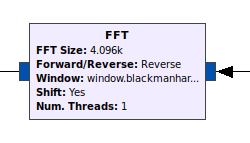
\includegraphics[scale=0.5]{figuras/cap05/fft}
	\caption{\label{f:fft} Bloque que implementa el algoritmo FFT.}
\end{figure}

El parámetro \textit{Reverse} del bloque, indica la dirección en la que se realiza la transformación. Dado que venimos trabajando en el dominio de la frecuencia y vamos a pasar al dominio temporal, debemos ejecutar el algoritmo en el sentido inverso.

\section{El prefijo cíclico}

Para sincronizar los relojes de transmision y recepción, y eliminar de forma suficiente la interferencia intersimbolica, es que en ISDBT se utiliza un prefijo cíclico. Esto es, las primeras N muestras de la señal, se copian tal cual están hacia el final de la señal. Esto hace que, al calcular la autocorrelacion de la señal en recepción, sea posible detectar de forma perfecta el comienzo de la señal, así como los parámetros de transmision en caso de que sean desconocidos. 

Se repaso el fundamento teorico detras de esta practica en el capitulo 3, en caso de buscar profundizar en la misma, una clara explicación de estos conceptos esta en \cite{gr-isdbt}. No entraremos en mas detalles de este proceso para no ser repetitivos.

\begin{figure}[!h]
	\centering
	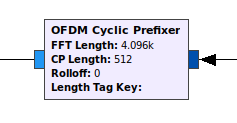
\includegraphics[scale=0.5]{figuras/cap05/cp}
	\caption{\label{f:cp} Bloque que implementa prefijo cíclico.}
\end{figure}

Este bloque tampoco es desarrollo propio del proyecto gr-isdbt-tx. Si bien escribimos un bloque que realiza esta funcionalidad (a nivel de programación se resuelve con un memcpy) preferimos dejar la implementacion existente, que funciona muy bien y esta validada por la comunidad de usuarios de GNU Radio.

De todos modos, la implementacion de este bloque es un problema que los tutores nos plantearon al inicio del proyecto, y es interesante como primer acercamiento al entorno de desarrollo de GNU Radio. La lógica detrás del funcionamiento del bloque es simple, por lo que el kid de la cuestión esta en manejar debidamente el movimiento de muestras entre el bloque y el core del software.

\section{La transmision desde USRP}

Como ya se discutió en secciones anteriores, para realizar la transmisión de la señal a través del equipo USRP, es necesario utilizar el bloque sink del complemento \textit{gr-uhd}. Siempre que se mantengan las condiciones para la buena transmision que se enumeraron en el capitulo 4, es esperable tener a la señal en el aire sin mayores problemas. 

Como consideraciones generales, recomendamos verificar que el espectro a utilizar este disponible, de forma de no solaparse con la señal de alguno de los canales comerciales, que transmiten a alta potencia y podrían causar problemas para decodificar nuestra señal.

Durante el desarrollo del transmisor, antes de probar la transmision contra un televisor comercial, una prueba bastante sencilla es la de transmitir hacia un archivo. Luego, podemos usar ese archivo como entrada de datos al receptor \textit{gr-isdbt} para corroborar que la transmision tenga todos los parámetros correctos. Disponer de todos los bloques del receptor para tomar medidas, es un excelente método de debugging.